\documentclass[a4paper,12pt]{article}

\usepackage{tikz}
\usetikzlibrary{decorations.pathreplacing}
\usepackage{amsmath}
\usepackage{amsfonts}
\usepackage{amssymb}
\usepackage[margin=1in]{geometry}
\usepackage{graphicx}
\usepackage[]{geometry}
\usepackage{inconsolata}
\usepackage{courier}
\usepackage{listings}
\usepackage{enumerate}
\usepackage{float}
\usepackage{answers}
\usepackage[english]{babel}
\usepackage{commath}
\usepackage[labelfont=bf]{caption}
\usepackage{mwe}
\usepackage[longnamesfirst]{natbib}
\usepackage{algorithm}
\usepackage[noend]{algpseudocode}
\usepackage{eurosym}
\usepackage{siunitx}
\usepackage{ctable}
\usepackage{subfig}
\usepackage{dsfont}

\setlength{\parindent}{0pt}
\setlength{\parskip}{1em}

\title{Maintenance Policies for a Multi-Unit System with Adjustable Production Rates}
\author{Mark van der Broek}
\date{\today}

\begin{document}
	
	\maketitle

\section{Introduction}	
% Good maintenance policies are required

% For systems with multiple units, there exists dependence between the units. 

% Windmills require expensive fixed costs, so clustering maintenance can be profitable. In many windmill contracts a specified production has to be met for the total windpark. Try to combine production with maintenance policies.



The system also allows to adjust the production rate of each unit, which has an impact on the deterioration process of the unit. The units deteriorate independently of each other, and we can perfectly observe this deterioration level for each unit at any moment in time. An graphical overview of the order of events within a time epoch is presented in Figure 1.



For the analysis I will consider a system of two units, and if time permits we will relax this assumption to consider a system with more units. For the maintenance policy can perform maintenance or not with cost $c_\text{pm}$ if the unit has not failed yet and cost $c_\text{cm}$ if it has failed. The cost of preventive maintenance is assumed to be less than corrective maintenance cost ($c_\text{pm} < c_\text{cm}$). Furthermore, for any time period we do perform maintenance a fixed cost $C$ has to be incurred. Therefore, depending on the size of these three costs it could be beneficial to cluster the maintenance actions.

\section{Markov Decision Process}
In this section we provide the Markov Decision Process (MDP) formulation of our problem. At the start of a time unit, the system can be in a certain state. Based on this current state, a set of maintenance actions can be performed. For each unit, this set consists of doing nothing or performing maintenance. After selecting the maintenance action, we set the production rate of each unit. Based on the current state, maintenance and production action for a time period, each unit of the system deteriorates according to some transition probabilities. A schematic overview of these processes within a time unit are presented in Figure \ref{timeline}. In this section we will specify the state space, action space, transition probabilities and the expected costs.

\begin{figure}[H]
	\centering
	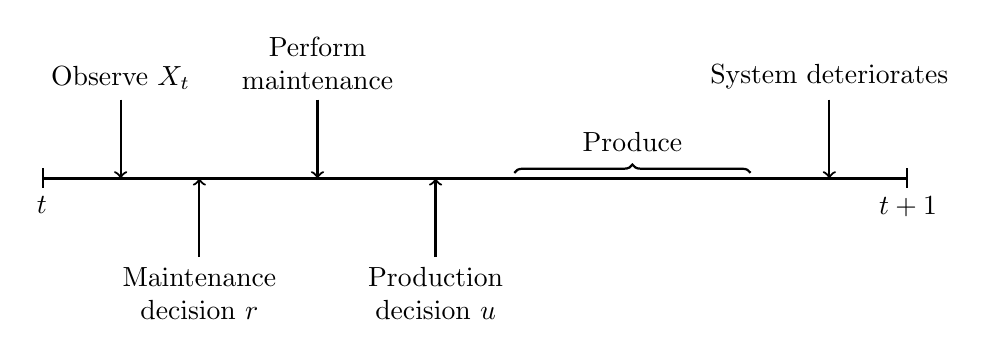
\begin{tikzpicture}
	\coordinate (t) at (0,0);
	\coordinate (X) at (1,0);
	\coordinate (R) at (2,0);
	\coordinate (M) at (3.5,0);
	\coordinate (U) at (5,0);
	\coordinate (UE) at (9,0);
	\coordinate (D) at (10,0);
	\coordinate (t+1) at (11,0);
	
	% Draw the time horizon
	\draw[thick, |-|] (t) -- (t+1);
	\draw (t) node[below=3pt] {$t$};
	\draw[thick, ->] (1,1) node[above, align=center] {Observe $X_t$} -- (X);
	\draw[thick, ->] (2,-1) node[below, align=center] {Maintenance \\ decision $r$} -- (R);
	\draw[thick, ->] (3.5, 1) node[above, align=center] {Perform \\ maintenance} -- (M);
	\draw[thick, ->] (5, -1) node[below, align=center] {Production \\ decision $u$} -- (U);
	\draw[thick, decorate, decoration={brace,raise=2pt, amplitude=3pt}] (6,0) -- (9, 0) node[sloped,midway, above=6pt] {Produce};
	\draw[thick, ->] (10, 1) node[above, align=center] {System deteriorates} -- (D);
	\draw (t+1) node[below=3pt] {$t+1$};
	\end{tikzpicture}
	\caption{Order of events for time epoch $t$.}
\end{figure}

\subsection{State space}
We consider a multi-unit system that consists of $n$ identical units. We denote the set of units as $\mathcal{I} = \{1, \dots, n\}$. Each unit deteriorates according to a discrete-time Markov chain with deterioration states $X = \{0, 1, \dots, L\}$. State $0$ represents the as-good-as-new state and state $L$ the failed state. The whole state of all units is denoted by
$$
x = (x_1, \dots, x_n) \in X^n.
$$

\subsection{Action space}
At the start of each time unit we have to decide on which components to maintain (M) and do nothing (DN). Maintenance can be performed one all units, independent of the current state, i.e., the action space for the maintenance decision can be defined as
$$
R = \left \{r = (r_1, \dots, r_n): r_i \in \{\text{DN}, \text{M}\}, \enskip \forall i \in \mathcal{I} \right \}.
$$

After selecting the maintenance action, we also have to set the production rate of each unit. Each unit can produce at most $m+1$ different production rates, ranging from $0$ to $1$ (maximum production). The possible production rates are uniformly distributed over the interval. If a unit is in the failed state, we cannot produce, so the production rate of this unit is set to $0$. For all other deteriorating levels, we can select one of the $m+1$ production rates. We define the set of possible production rates for unit $i$ in state $x_i$ $U(x_i)$ as follows
$$
U(x_i) = \begin{cases}
\{0, 1/m, \dots, 1\} & \text{ if } x_i \neq L, \\
\{0\} & \text{ if } x_i = L.
\end{cases}
$$
Hence, the 
Let $u = (u_1, \dots, u_n)$ denote the production rate of all units in the system. The total production of the system is restricted to $\pi$, i.e., $ \sum_{i=1}^{n}u_i = \pi$. This results in the following action space for the system in state $x$
$$
U(x) = \left\{ u  :  \sum_{i=1}^{n}u_i = \pi, u_i \in U(x_i) \enskip \forall i \in \mathcal{I} \right\}.
$$
Note that the production action space decreases from $(m+1)^n$ elements to ${n + \pi - 1} \choose{\pi - 1} $ by restriction the total production rate to the value $\pi$. 

\subsection{Deterioration Process}
The transition probabilities for all units are identical and independent. Each unit $i$ deteriorates according to a gamma process with rate $\lambda(u_i)$, which depends on the current production rate of the unit, and variance $\sigma^2$. The rate for a given production rate $u_i$ is given by
$$
\lambda(u_i) = g(u_i) \lambda_{\text{max}},
$$
where $\lambda_{\text{max}}$ is the rate parameter under the maximum production rate, and $g$ is some non-decreasing function. We assume that $g(u_i)$ as a function of the production rate $u_i$ for unit $i$ is of the following form
$$
g(u_i) = \beta + (1-\beta)u_i^\alpha.
$$
We assume that $0 \leq \beta \leq 1$ and $\alpha \geq 0$, since $g$ should be non-decreasing in $u_i$. \textbf{[[Add some information about the shape of $g$]]}

For a unit $i$ the probability of having $q \geq 0$ jumps in the deterioration states for a time epoch under production rate $u_i$ is given by $p(u_i,q)$, which can be found by discretising the gamma process (see De Jonge). The transition probability of unit $k$ for going from state $i$ to $j$ with production rate $u_i$ and maintenance action DN for any time epoch is defined as
$$
P_{u_k,\text{DN}}(i,j) = \begin{cases}
p(u_k, j-i) &\text{ if } i \leq j \leq L-1, \\
0 &\text{ if } j < i, \\
1 - \sum_{l=0}^{L-1-i}p(u_k,l) & \text{ if } i \leq m-1  \text{ and } j = L, \\
1 & \text{ if } i = j = L,
\end{cases}
$$
and for maintenance action M by
$$
P_{u_k,\text{M}}(i,j) = \begin{cases}
p(u_k, j) &\text{ if } j \leq  L-1, \\
1 - \sum_{l=0}^{L-1}p(u_k,l) & \text{ if } j = L.
\end{cases}
$$
Note that for the maintenance action M the probability of going from state $i$ to $j$ does not depend on $i$, since we assume that the system will go to state 0 immediately after the maintenance action.

The transition probability of a unit in the system is independent of the other units. Therefore, the transition probability that the system goes from state $x = (x_1, \dots, x_n)$ to state $\tilde{x} = (\tilde{x}_1, \dots, \tilde{x}_n)$ by selecting production rates $u$ and maintenance actions $m$ is given by
$$
p(x, \tilde{x} \mid u, m) = \prod_{i = 1}^nP_{u_i,m_i}(x_i, \tilde{x}_i),
$$
due to independence of the deterioration process of the units.


\subsection{Expected costs}
To define the cost for a time unit, we define a function
$$
c(x_i,r_i) = \begin{cases}
c_{\text{pm}} & \text{ if } r_i = \text{M} \text{ and } x_i \neq L, \\
c_{\text{cm}} & \text{ if } r_i = \text{M} \text{ and } x_i = L, \\
0 & \text{ elsewhere}.
\end{cases}
$$
for all states $x_i \in X$ and maintenance actions $r_i \in \{\text{DN}, \text{M}\}$ of unit $i \in \mathcal{I}$. This means that if unit $i$ is in the failed state and we decide to perform maintenance, we incur the corrective maintenance costs $c_{\text{cm}}$, and if the unit has not failed, then the preventive maintenance costs $c_{\text{pm}}$ is incurred. 

The expected costs for a time unit by selecting maintenance action $r$ and in state $x$ is given by
$$
\bar{c}(x,r) = \begin{cases}
C + \sum_{i=1}^{n}c(x_i, r_i), &\text{if } r \text{ contains a maintenance action},\\
0, &\text{otherwise}.
\end{cases}
$$
In words, this means that if we do not perform maintenance on any unit for a given time period, we do not incur any costs. However, if we do perform maintenance, we incur the fixed cost $C$ and some corrective or preventive costs depending on the state of the maintained unit.
\subsection{Performance criteria}
As a performance criterion, we are interested in minimizing the long-run average cost per time unit. In this way, we can quantify the impact of adding an additional component, and find the most cost-efficient maintenance policy. 

\section{Numerical results}

\subsection{Two unit setting}

\subsection{Adding additional unit}
\begin{enumerate}
	\item Directly compare the results for different mean rates $g$. 
\end{enumerate}

\subsection{Benchmark policies}
Since the action space of our problem consists of a maintenance action and a production action, we distinguish between a benchmark for the maintenance action and the production action. 

In the literature, condition-based maintenance is often implemented in the form of a threshold policy (CITE). Due to the economic dependence (fixed cost of maintenance) and the liberty to set the production rate of the components, this policy is probably not optimal. For this policy, if the deterioration level of a unit is at or exceed a threshold level $T_r$, we perform a maintenance action. We find the optimal $T_r$ by simulating the system for a grid of values for $T_r$.

Production benchmark ideas:
\begin{enumerate}
	\item Share production equally between all units for all states.
	\item Random pool of $n$ units that produce equal amount.
	\item Best 50\% produces 80\% and worst 50\% 20\%.
\end{enumerate}

\subsection{Sensitivity analysis}
\begin{enumerate}
	\item Effect of fixed costs. More or less clustered maintenance.
	\item Effect of variance.
	
\end{enumerate}

\appendix

\section{Appendix}

\subsection{Discretising the gamma process}


